\documentclass{beamer}

\newcommand*\whitem{%
  \item[\color{white}\scalebox{0.9}{\textbullet}]}

\mode<presentation>
{
  \usetheme{Singapore}
  \renewcommand{\insertnavigation}[1]{}
  \setbeamercovered{transparent}
}

\usepackage[english]{babel}
\usepackage[absolute,overlay]{textpos}
\usepackage[latin1]{inputenc}
\usepackage{times}
\usepackage{graphicx}
\usepackage{epstopdf}
\usepackage[T1]{fontenc}
\usepackage{soul}
\usepackage{pdflscape}
\usepackage{multirow}

\beamertemplatenavigationsymbolsempty

\newcommand{\citations}[1]
   {
     \begin{textblock}{16}[1,1](15.75,15.25)
       \flushright{\scriptsize #1}
     \end{textblock}
   }

\definecolor{MedPurple}{RGB}{194,165,207}
\definecolor{DeepPurple}{RGB}{118,42,131}
\definecolor{LightGreen}{RGB}{166,219,160}
\definecolor{DarkGreen}{RGB}{0,68,27}
\definecolor{MedGreen}{RGB}{90,174,97}
\definecolor{DarkBlue}{RGB}{0,68,127}

\setbeamercolor{title}{fg=DeepPurple} % Main title text
\setbeamercolor{frametitle}{fg=DeepPurple} % Panel title text
\setbeamercolor{structure}{fg=DarkBlue} % Panel header

\setbeamercolor{*}{bg=3}

\title[Do motif roles predict species responses to perturbations?]
{Do motif roles predict\\ species responses to perturbations?}

\author[A.R. Cirtwill \& K. Wootton]{\textbf{Alyssa R. Cirtwill} \& Kate Wootton} 

\date[Short Occasion]
{4th Symposium on Ecological Networks\\13/09/2019}

% \institute{Stockholm University, Swedish Agricultural University (SLU)}%\\[\smallskipamount]
  % \hspace{-1cm} 
\includegraphics[width=.2\textwidth,height=.2\textwidth]{intro_figs/SU_logo.eps} \hspace{2cm} 
\includegraphics[width=.3\textwidth,height=.3\textwidth]{intro_figs/SLU_logo.eps}}

\titlegraphic{ \vspace{-1cm}

\includegraphics[width=.2\textwidth]{intro_figs/SU_logo.eps} \hspace{5.7cm} 
\includegraphics[width=.25\textwidth]{intro_figs/SLU_logo.eps} 
}


\subject{Talks}

\begin{document}

\newcommand{\SubItem}[1]{
    {\setlength\itemindent{12pt} \item[*] #1}
}

\begin{frame}
  \titlepage
\end{frame}

\section*{Introduction} % Figs done, update facts

    % \begin{frame}{Ecological networks}
    %   \begin{textblock*}{10cm}(1cm,1.5cm)
    %     Ecological networks:
    %     \begin{itemize}
    %       \item Connect species, map (trophic) interactions
    %     \end{itemize}
    %     \end{textblock*}
    %   \begin{textblock*}{5cm}(1cm,5cm)
    %     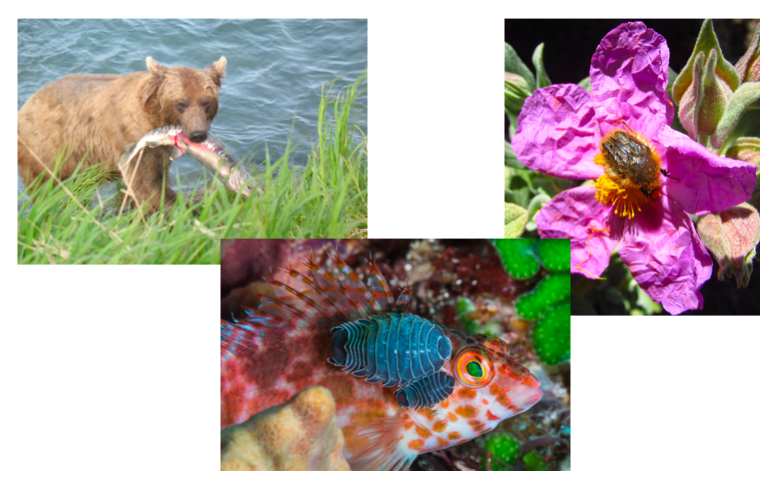
\includegraphics[width=5cm]{intro_figs/interaction_examples.eps}
    %     \end{textblock*}
    %   \begin{textblock*}{5cm}(7cm,4cm)
    %     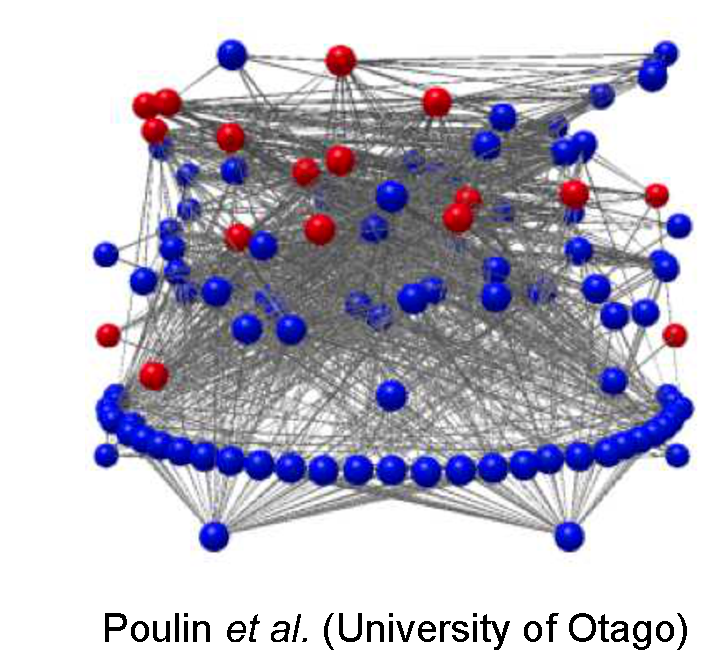
\includegraphics[width=5cm]{intro_figs/Otagoweb.eps}
    %     \end{textblock*}        
    %   \end{frame}

    % \begin{frame}{Ecological networks}
    %   \begin{textblock*}{10cm}(1cm,1.5cm)
    %     Ecological networks:
    %     \begin{itemize}
    %       \item Connect species, map (trophic) interactions
    %       \begin{itemize}
    %         \item  Direct \& indirect interactions
    %       \end{itemize}
    %     \end{itemize}
    %     \end{textblock*}
    %   \begin{textblock*}{5cm}(1cm,5cm)
    %     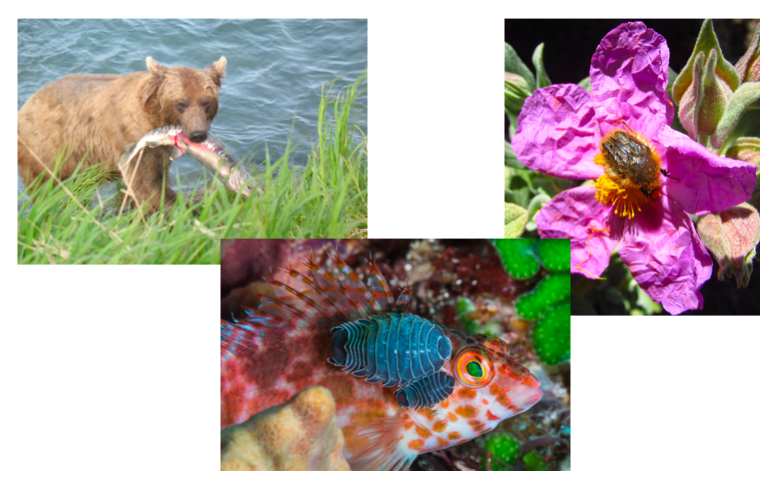
\includegraphics[width=5cm]{intro_figs/interaction_examples.eps}
    %     \end{textblock*}
    %   \begin{textblock*}{5cm}(7cm,4cm)
    %     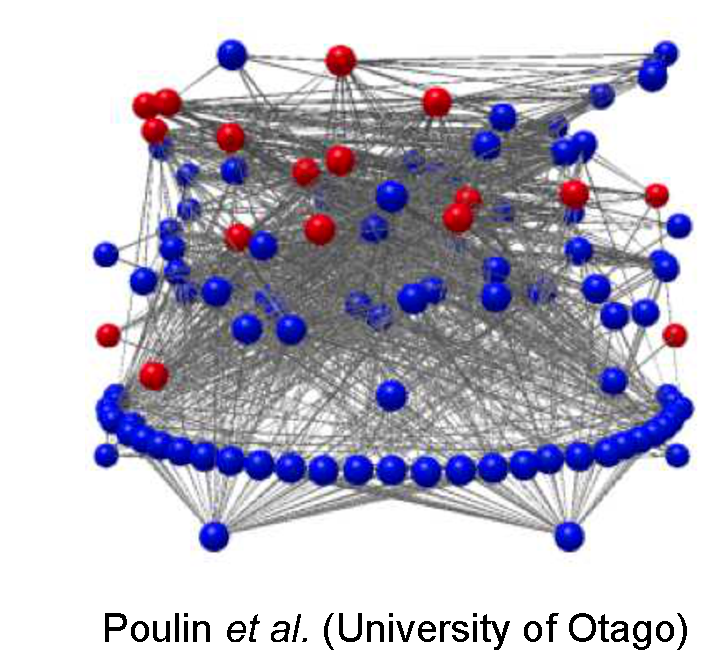
\includegraphics[width=5cm]{intro_figs/Otagoweb.eps}
    %     \end{textblock*}        
    %   \end{frame}

    % \begin{frame}{Ecological networks}
    %   \begin{textblock*}{10cm}(1cm,1.5cm)
    %     Ecological networks:
    %     \begin{itemize}
    %       \item Connect species, map (trophic) interactions
    %       \begin{itemize}
    %         \item  Direct \& indirect interactions
    %       \end{itemize}
    %       \item Predict community stability \& function
    %     \end{itemize}
    %     \end{textblock*}
    %   \begin{textblock*}{5cm}(1cm,5cm)
    %     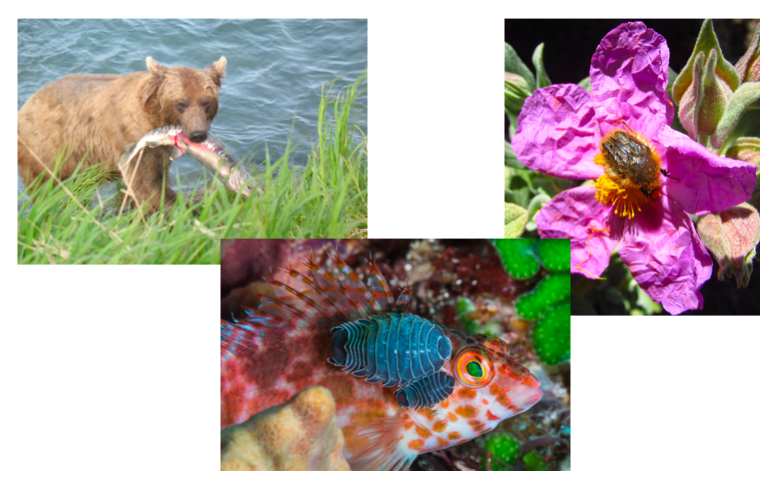
\includegraphics[width=5cm]{intro_figs/interaction_examples.eps}
    %     \end{textblock*}
    %   \begin{textblock*}{5cm}(7cm,4cm)
    %     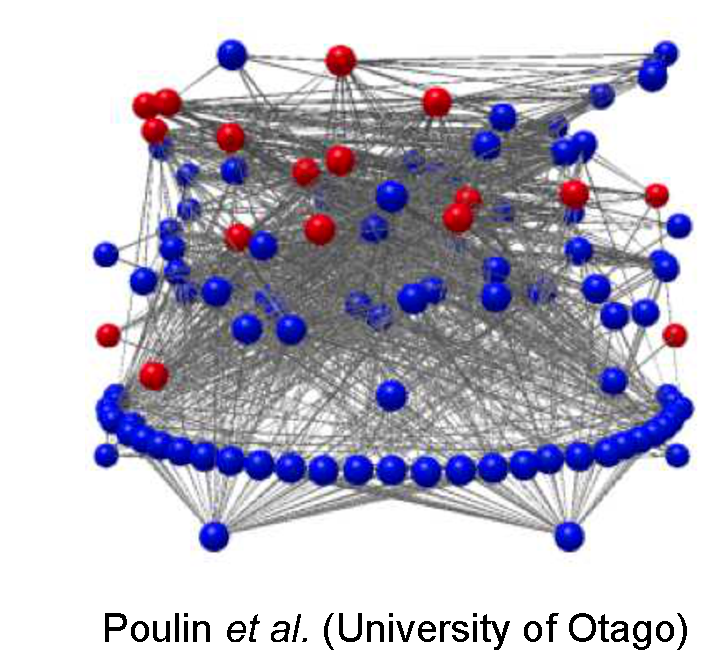
\includegraphics[width=5cm]{intro_figs/Otagoweb.eps}
    %     \end{textblock*}        
    %   \end{frame}

    % \begin{frame}{Ecological networks}
    %   \begin{textblock*}{10cm}(1cm,1.5cm)
    %     Ecological networks:
    %     \begin{itemize}
    %       \item Connect species, map (trophic) interactions
    %       \begin{itemize}
    %         \item  Direct \& indirect interactions
    %       \end{itemize}
    %       \item Predict community stability \& function
    %       \begin{itemize}
    %         \item Robustness
    %         \item Resilience
    %       \end{itemize}
    %     \end{itemize}
    %     \end{textblock*}
    %   \begin{textblock*}{5cm}(1cm,5cm)
    %     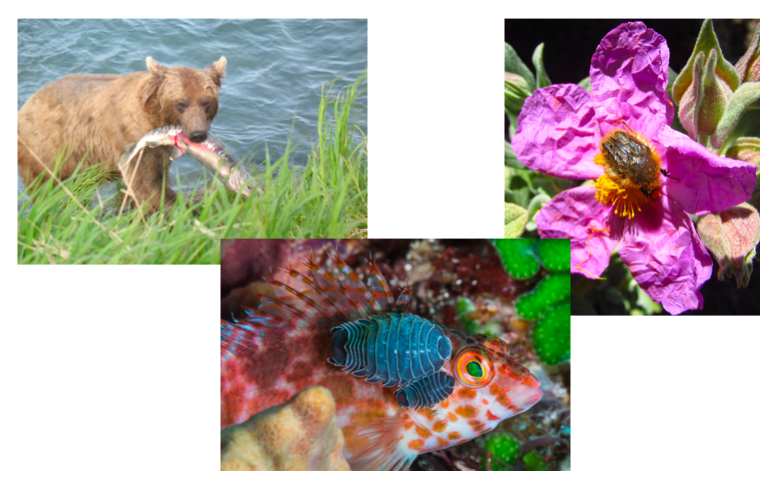
\includegraphics[width=5cm]{intro_figs/interaction_examples.eps}
    %     \end{textblock*}
    %   \begin{textblock*}{5cm}(7cm,4cm)
    %     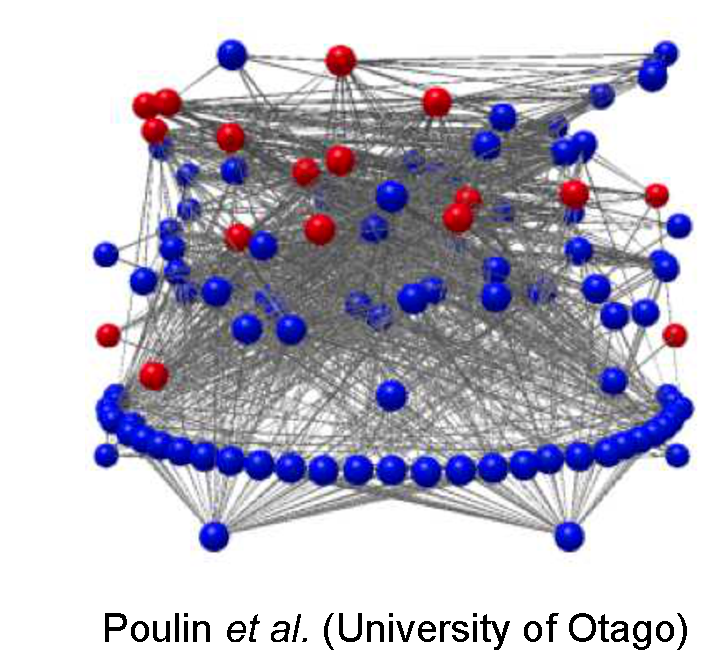
\includegraphics[width=5cm]{intro_figs/Otagoweb.eps}
    %     \end{textblock*}        
    %   \end{frame}

    \begin{frame}{A species-eye view of ecological networks}
      \begin{textblock*}{10cm}(1cm,1.5cm)
        Ecological networks:
        \begin{itemize}
          \item Connect species, map interactions
          \item Predict community stability \& function
          \whitem {\color{white}Hard to see species differences}
        \end{itemize}
        \end{textblock*}
      \begin{textblock*}{5cm}(1cm,5cm)
        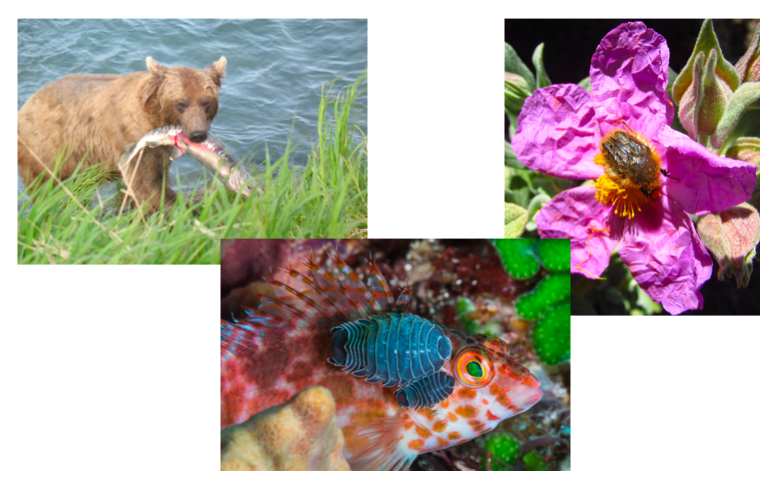
\includegraphics[width=5cm]{intro_figs/interaction_examples.eps}
        \end{textblock*}
      \begin{textblock*}{5cm}(8cm,3.25cm)
        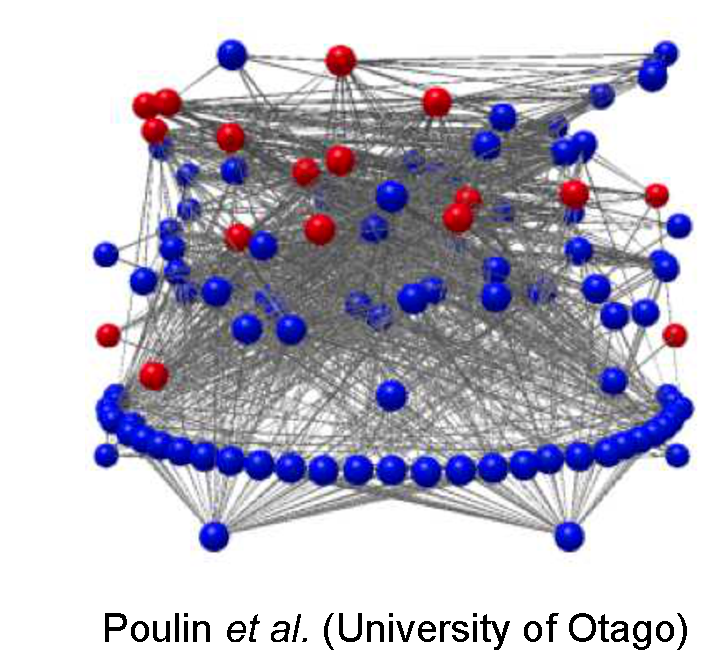
\includegraphics[width=4cm]{intro_figs/Otagoweb.eps}
        \end{textblock*}    
      \end{frame}

    % \begin{frame}{Ecological networks and stability}
    %   \begin{textblock*}{9cm}(0.5cm,2cm)
    %     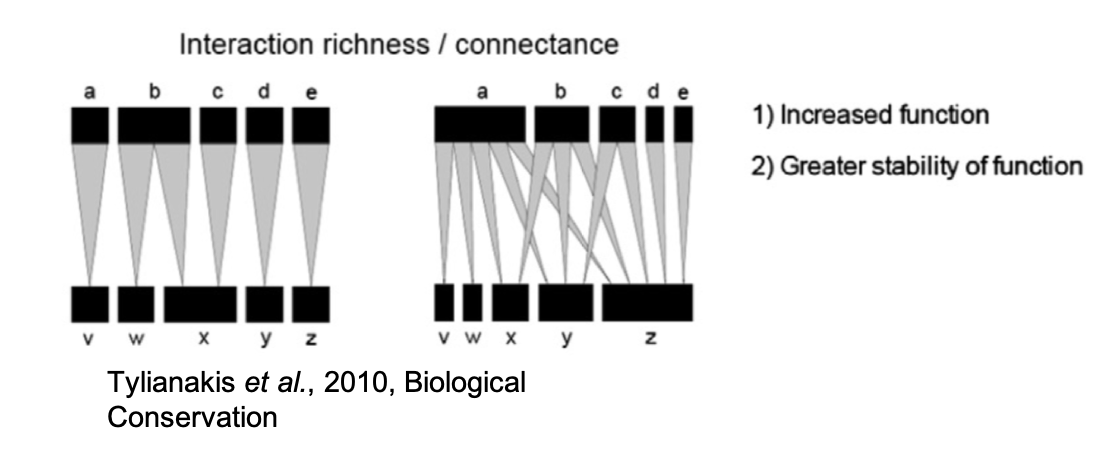
\includegraphics[width=8.5cm]{intro_figs/expanded_bipnet.eps}
    %     \end{textblock*}
    %   % \begin{textblock*}{9cm}(2cm,6cm)
    %   %   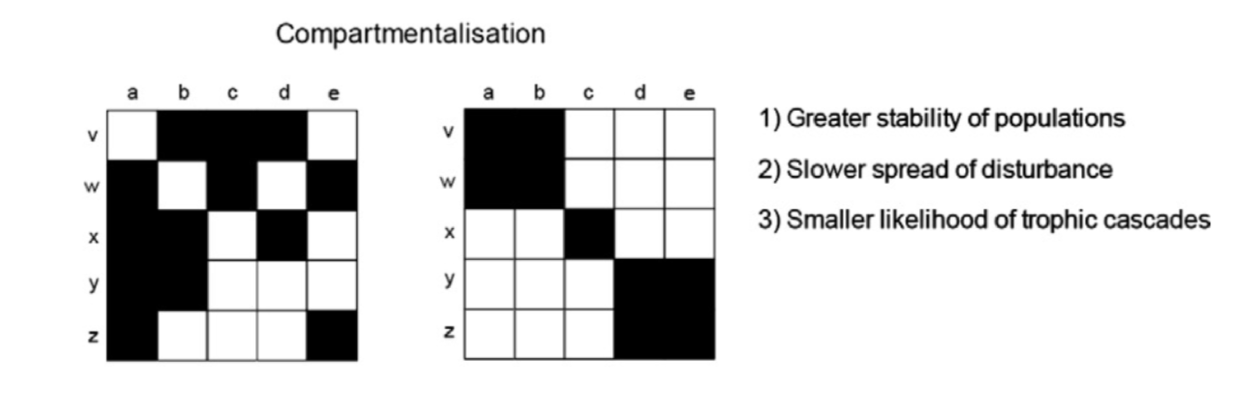
\includegraphics[width=8.5cm]{intro_figs/compartments.eps}
    %   %   \end{textblock*}
    %   \begin{textblock*}{5cm}(9.5cm,1.5cm)
    %     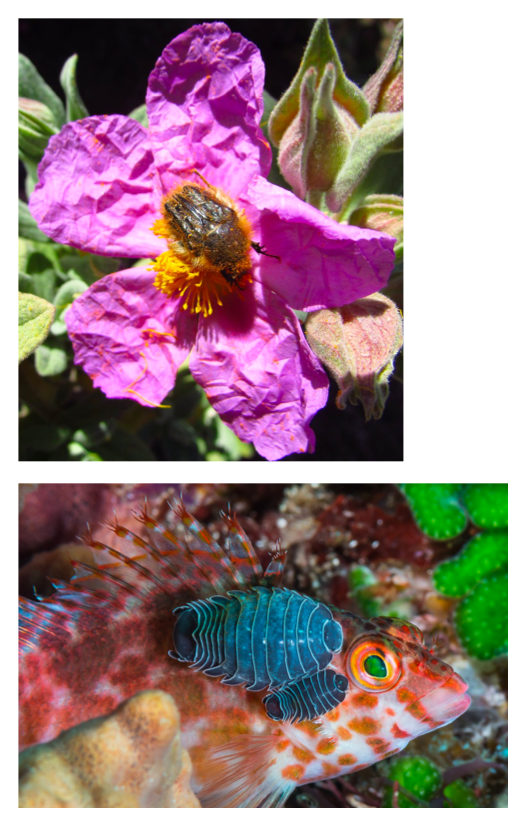
\includegraphics[width=3cm]{intro_figs/bipartite_examples.eps}
    %     \end{textblock*}        

    %   \end{frame}

    % \begin{frame}{Ecological networks and stability}
    %   \begin{textblock*}{9cm}(0.5cm,2cm)
    %     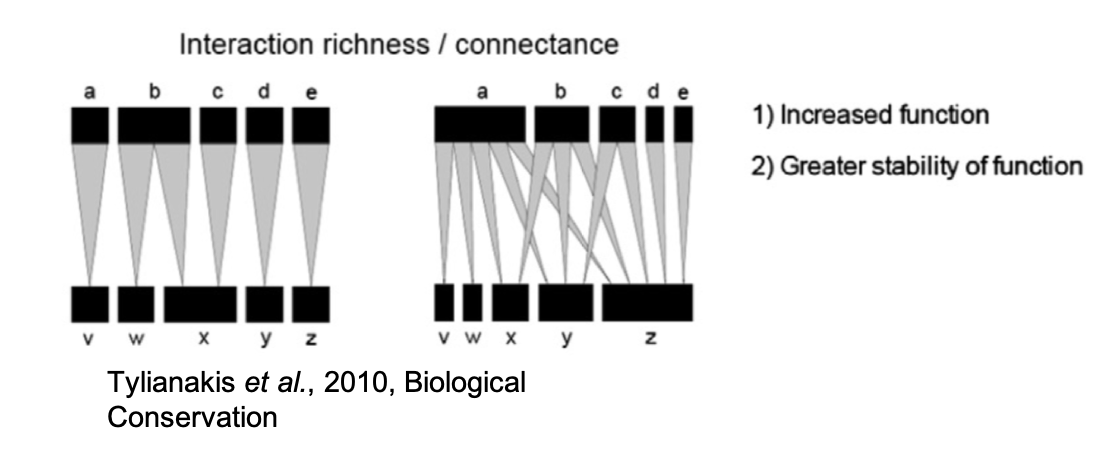
\includegraphics[width=8.5cm]{intro_figs/expanded_bipnet.eps}
    %     \end{textblock*}
    %   \begin{textblock*}{9cm}(2cm,6cm)
    %     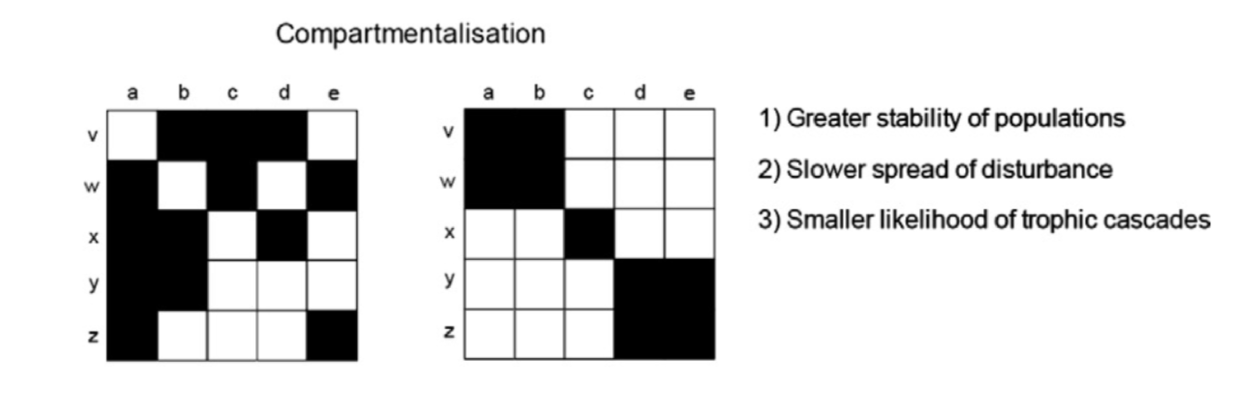
\includegraphics[width=8.5cm]{intro_figs/compartments.eps}
    %     \end{textblock*}
    %   \begin{textblock*}{5cm}(9.5cm,1.5cm)
    %     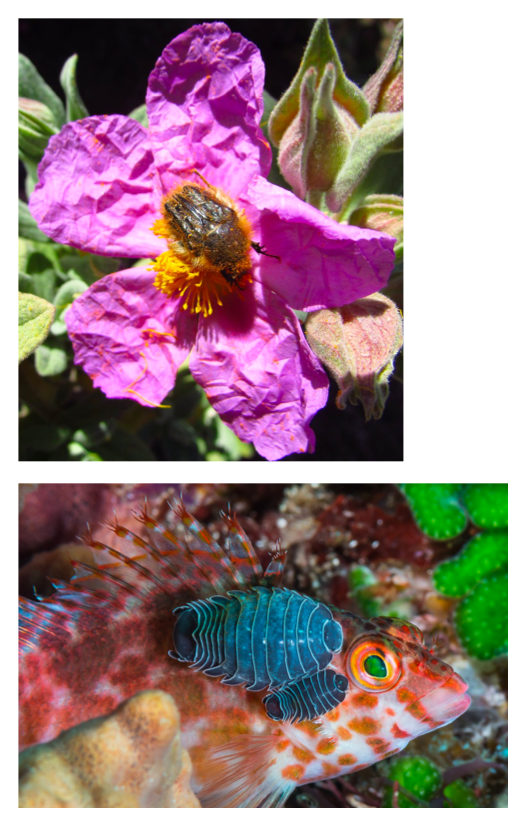
\includegraphics[width=3cm]{intro_figs/bipartite_examples.eps}
    %     \end{textblock*}        
    %   \end{frame}

    \begin{frame}{A species-eye view of ecological networks}
      \begin{textblock*}{10cm}(1cm,1.5cm)
        Ecological networks:
        \begin{itemize}
          \item Connect species, map interactions
          \item Predict community stability \& function
          \item Hard to see species differences
        \end{itemize}
        \end{textblock*}
      \begin{textblock*}{5cm}(1cm,5cm)
        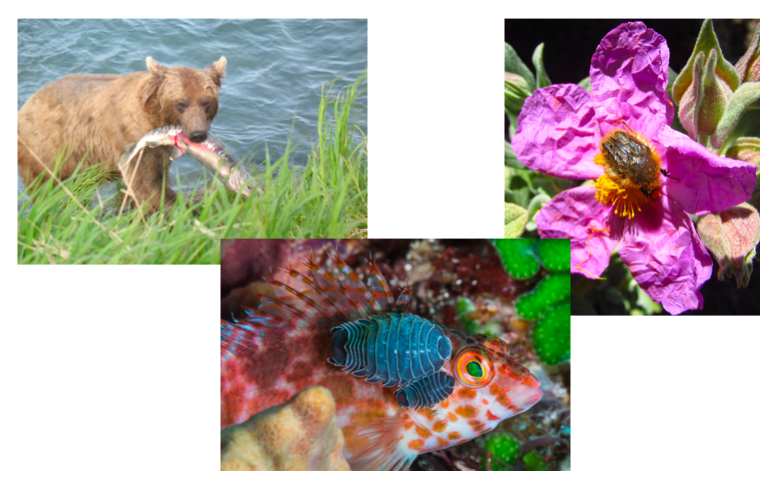
\includegraphics[width=5cm]{intro_figs/interaction_examples.eps}
        \end{textblock*}
      \begin{textblock*}{5cm}(8cm,3.25cm)
        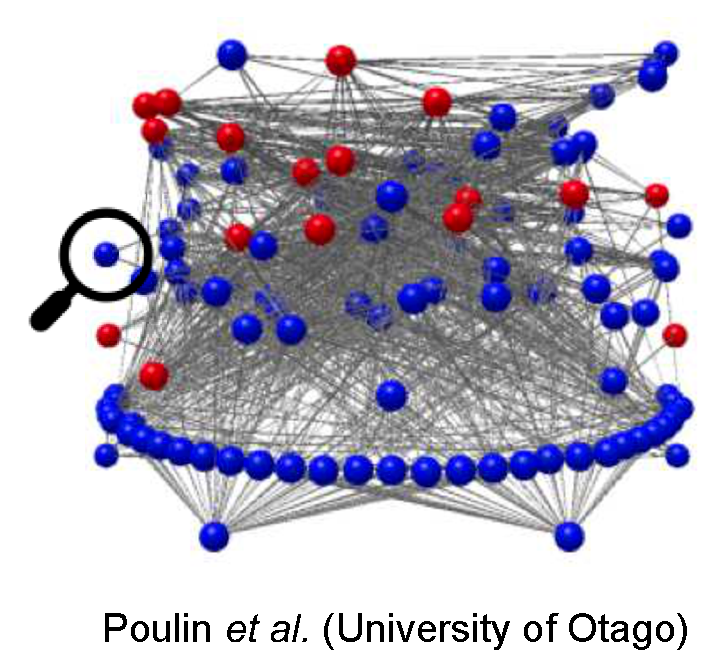
\includegraphics[width=4cm]{intro_figs/Otagoweb_closeup.eps}
        \end{textblock*}    
      \end{frame}

\section*{Motifs, roles, and stability}
  \begin{frame}{A species-eye view of ecological networks}
      \begin{textblock*}{10cm}(1cm,1.5cm)
        Ecological networks:
        \begin{itemize}
          \item Connect species, map interactions
          \item Predict community stability \& function
          \item Hard to see species differences
          \item Motifs to the rescue!
        \end{itemize}
        \end{textblock*}

      \begin{textblock*}{5cm}(8cm,3.25cm)
        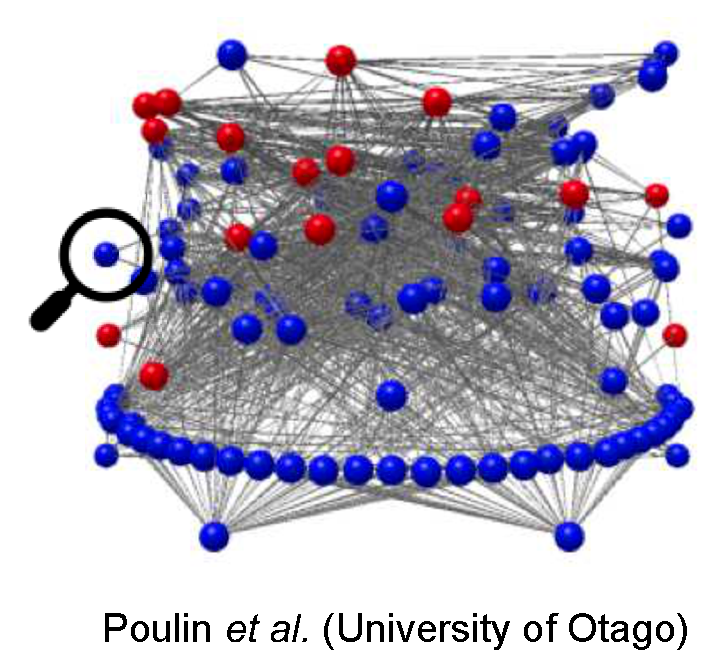
\includegraphics[width=4cm]{intro_figs/Otagoweb_closeup.eps}
        \end{textblock*} 

      \begin{textblock*}{7.5cm}(0.5cm,5.25cm)
        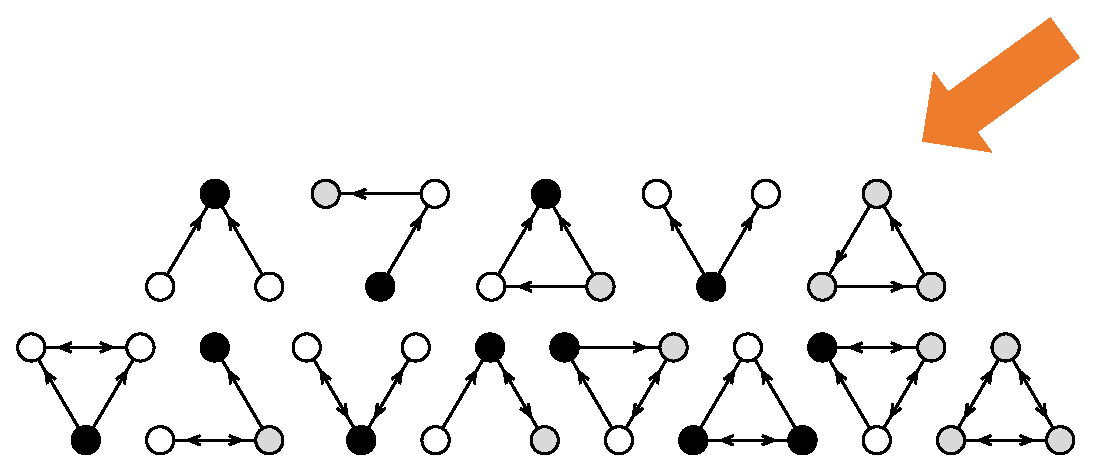
\includegraphics[width=7.5cm]{intro_figs/to_motifs.eps}
        \end{textblock*}       

    \end{frame}

  \begin{frame}{A species-eye view of ecological networks}

    % \begin{textblock*}{12cm}(0.5cm,5cm)
    %   \begin{center}
    %     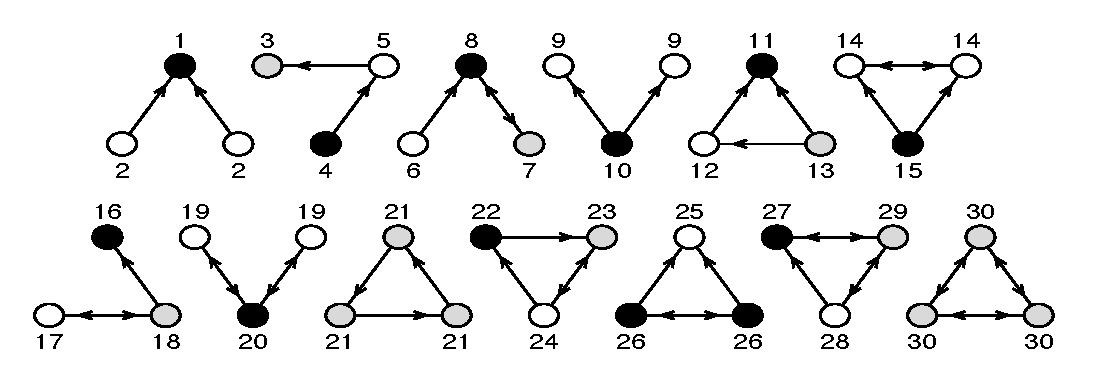
\includegraphics[width=9cm]{intro_figs/motifs_and_positions.eps}
    %     \end{center}       
    % \end{textblock*}

    \begin{textblock*}{12cm}(0.5cm,1.5cm)
      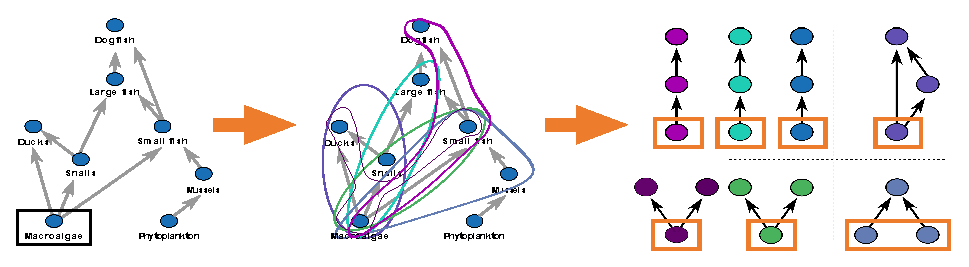
\includegraphics[width=12cm]{intro_figs/role_breakdown.eps}
      \end{textblock*} 

    \end{frame}

  \begin{frame}{A species-eye view of ecological networks}

    \begin{textblock*}{12cm}(0.5cm,1.5cm)
      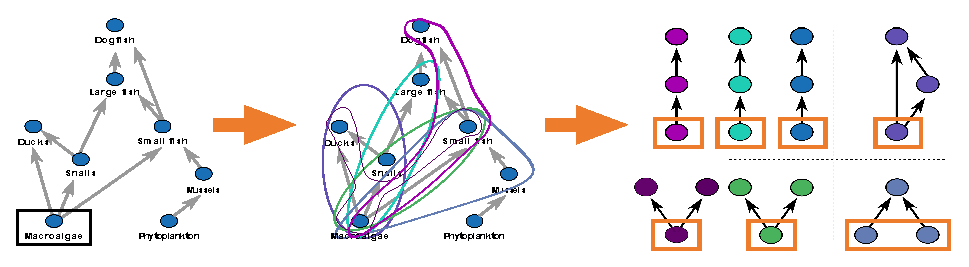
\includegraphics[width=12cm]{intro_figs/role_breakdown.eps}
      \end{textblock*} 

    \begin{textblock*}{6cm}(0.5cm,5cm)
      \begin{itemize}
        \item Compare parasites \& free-living species
        \item Link traits to network roles
        \item Track change over time
      \end{itemize}

      \vspace{.5cm}
      {\color{white}But what about prediction?}

      \end{textblock*} 

    \begin{textblock*}{6cm}(6.5cm,5cm)
        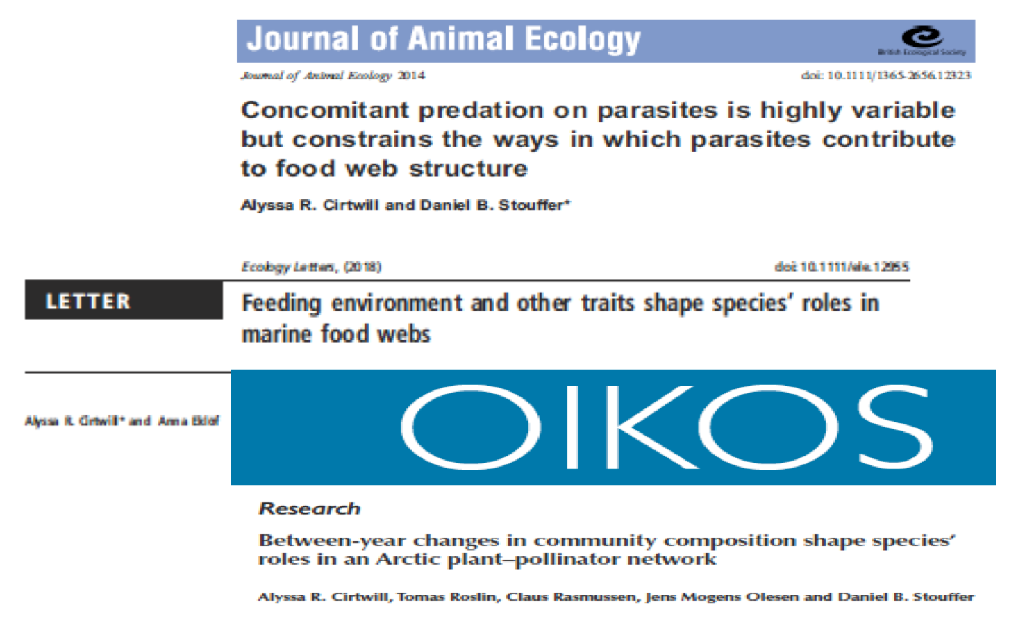
\includegraphics[width=0.8\textwidth]{intro_figs/paperstack.eps}
      \end{textblock*} 

    \end{frame}

  \begin{frame}{A species-eye view of ecological networks}

    \begin{textblock*}{12cm}(0.5cm,1.5cm)
      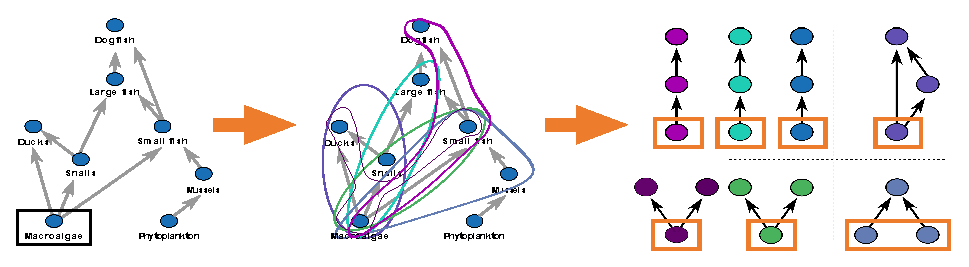
\includegraphics[width=12cm]{intro_figs/role_breakdown.eps}
      \end{textblock*} 

    \begin{textblock*}{6cm}(0.5cm,5cm)
      \begin{itemize}
        \item Compare parasites \& free-living species
        \item Link traits to network roles
        \item Track change over time
      \end{itemize}

      \vspace{.5cm}
      {\color{DarkBlue}But what about prediction?}

      \end{textblock*} 

    \begin{textblock*}{6cm}(6.5cm,5cm)
        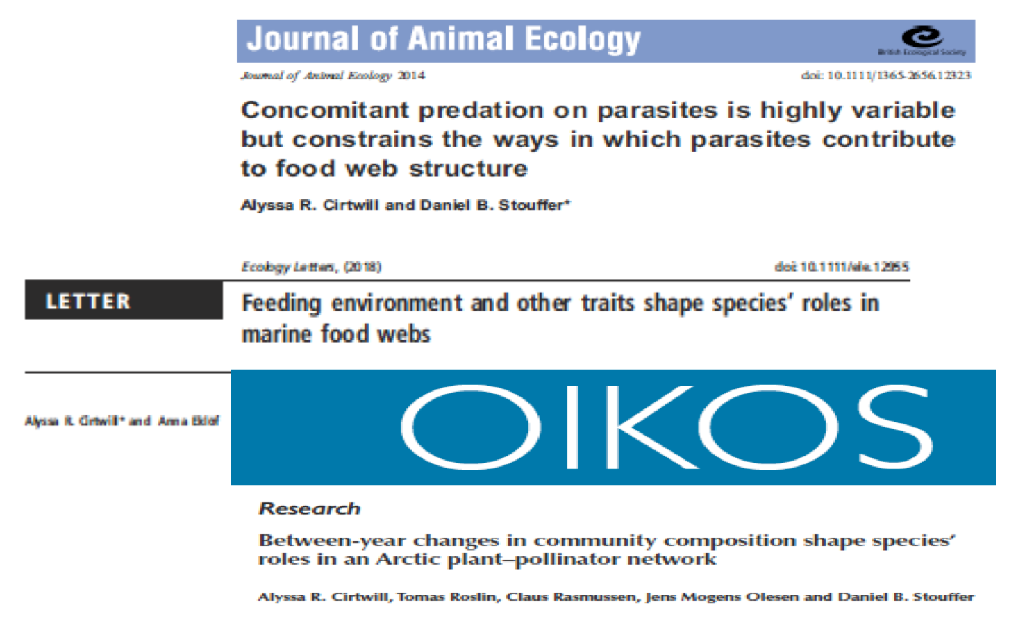
\includegraphics[width=0.8\textwidth]{intro_figs/paperstack.eps}
      \end{textblock*} 

    \end{frame}

  \begin{frame}{Linking motifs and stability to predict extinctions}

    \begin{textblock*}{12cm}(0.5cm,5cm)
      \begin{center}
        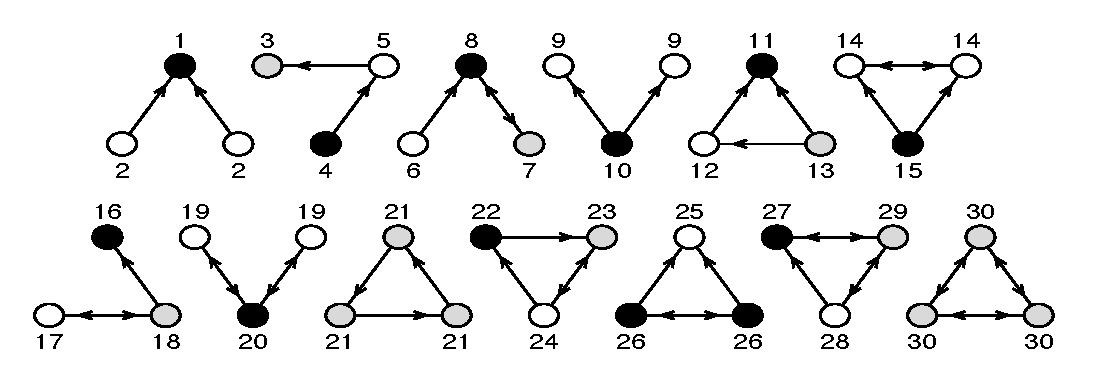
\includegraphics[width=9cm]{intro_figs/motifs_and_positions.eps}
        \end{center}       
    \end{textblock*}

    \begin{textblock*}{12cm}(0.5cm,1.5cm)
      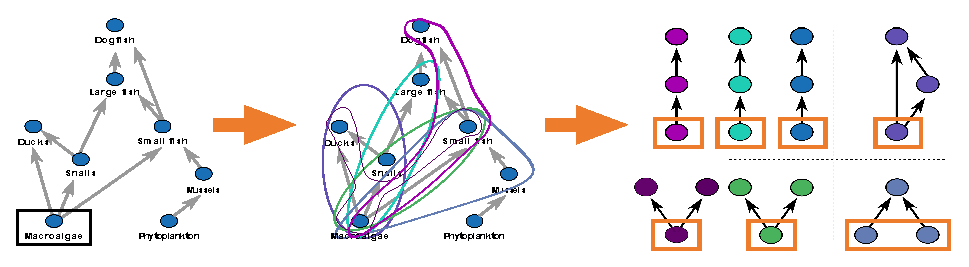
\includegraphics[width=12cm]{intro_figs/role_breakdown.eps}
      \end{textblock*} 

    \begin{textblock*}{12cm}(0.5cm,8.5cm)
      \begin{center}
        {\color{DarkBlue}Do some motifs stabilize the species within them?}
        \end{center}       
    \end{textblock*} 

    \end{frame}

  \begin{frame}{Linking motifs and stability to predict extinctions}

    \begin{textblock*}{12cm}(0.5cm,5cm)
      \begin{center}
        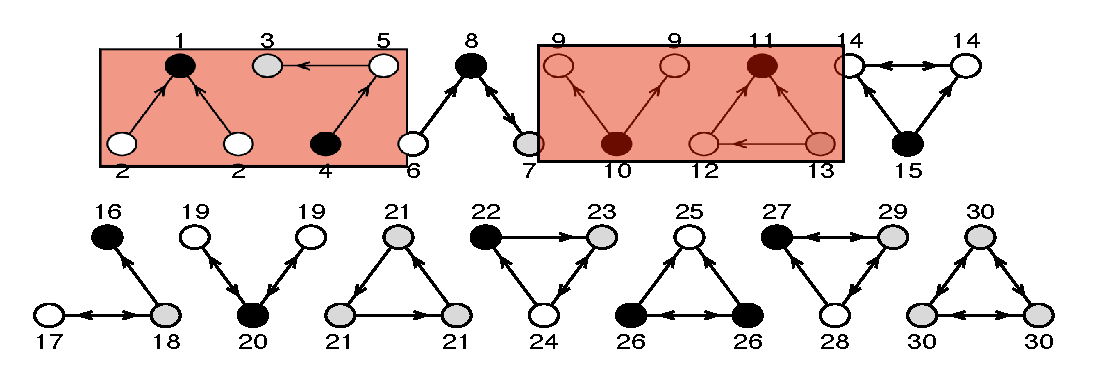
\includegraphics[width=9cm]{intro_figs/stable_motifs_and_positions.eps}
        \end{center}       
    \end{textblock*}     

      \begin{textblock*}{12cm}(0.5cm,1.5cm)
        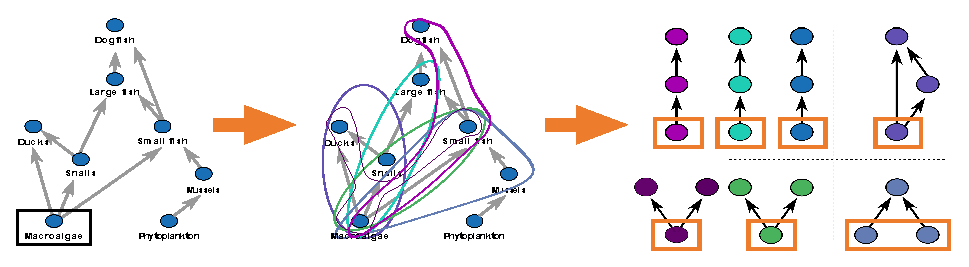
\includegraphics[width=12cm]{intro_figs/role_breakdown.eps}
        \end{textblock*} 

    \begin{textblock*}{12cm}(0.5cm,8.5cm)
      \begin{center}
        {\color{DarkBlue}Do some motifs stabilize the species within them?}
        \end{center}       
    \end{textblock*} 

    \end{frame}

  \begin{frame}{Linking motifs and stability to predict extinctions}
      \begin{textblock*}{10cm}(1cm,1.5cm)
        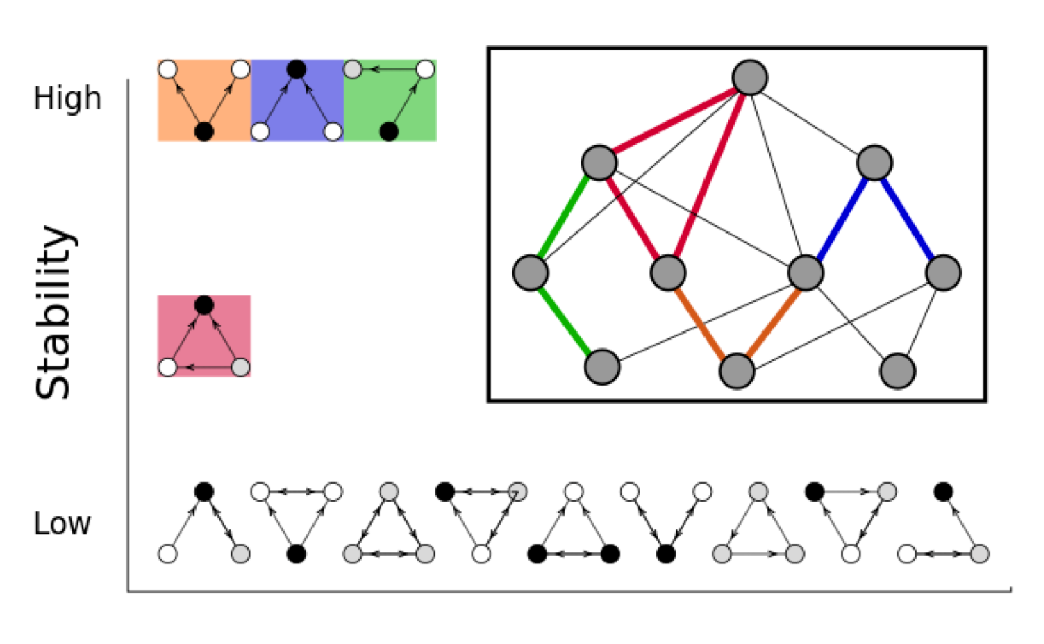
\includegraphics[width=10cm]{intro_figs/motifs_vs_stability.eps}
        \end{textblock*} 

      \begin{textblock*}{10cm}(1cm,7.5cm)
        \begin{itemize}
          \item More stable in isolation
          \whitem {\color{white}May help species in them to persist?}
        \end{itemize}
        {\tiny Results from Stouffer \emph{et al.} (2007) \textbf{Proc R Soc B} and Borelli (2015) \textbf{Oikos}}
        \end{textblock*}
    \end{frame}

  \begin{frame}{Linking motifs and stability to predict extinctions}
      \begin{textblock*}{10cm}(1cm,1.5cm)
        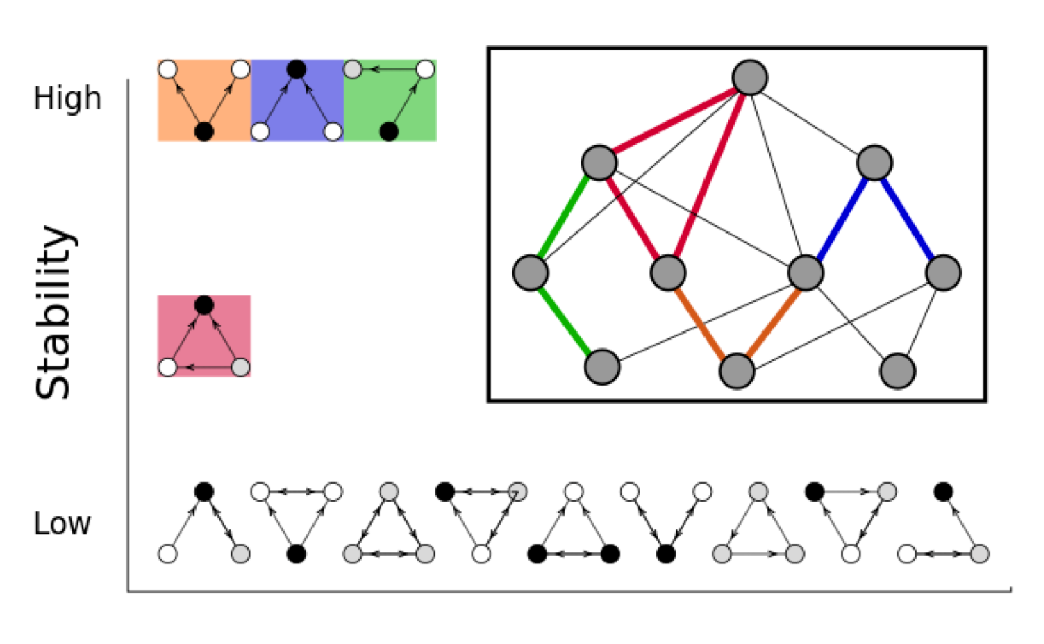
\includegraphics[width=10cm]{intro_figs/motifs_vs_stability.eps}
        \end{textblock*} 

      \begin{textblock*}{10cm}(1cm,7.5cm)
        \begin{itemize}
          \item More stable in isolation, associated with stable webs
          \whitem {\color{white}May help species in them to persist?}
        \end{itemize}
        {\tiny Results from Stouffer \emph{et al.} (2007) \textbf{Proc R Soc B} and Borelli (2015) \textbf{Oikos}}
        \end{textblock*}
    \end{frame}

  \begin{frame}{Linking motifs and stability to predict extinctions}
      \begin{textblock*}{10cm}(1cm,1.5cm)
        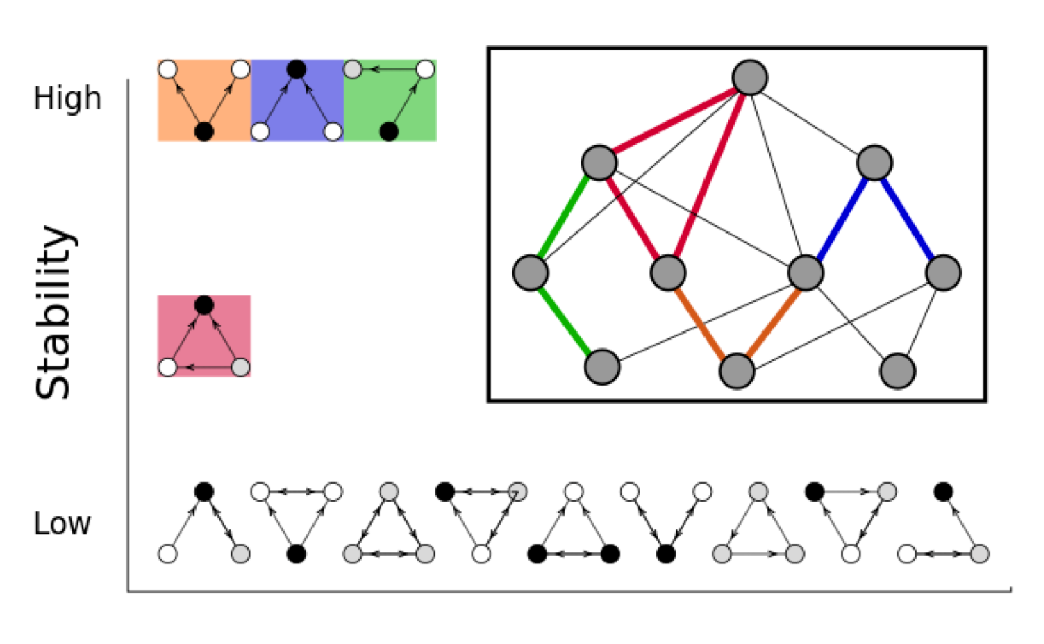
\includegraphics[width=10cm]{intro_figs/motifs_vs_stability.eps}
        \end{textblock*} 

      \begin{textblock*}{10cm}(1cm,7.5cm)
        \begin{itemize}
          \item More stable in isolation, associated with stable webs
          \item May help species in them to persist?
        \end{itemize}
        {\tiny Results from Stouffer \emph{et al.} (2007) \textbf{Proc R Soc B} and Borelli (2015) \textbf{Oikos}}
        \end{textblock*}
    \end{frame}

\section*{Methods: Network generation}
  \begin{frame}{Relating species roles to extinction risk}
      \begin{itemize}
        \item Simulated networks stable at equilibrium
        \item Webs with 50-100 species, connectance 0.02-0.2
        \item 100 simulated ATN networks for each combination
      \end{itemize}

      \begin{centering}

      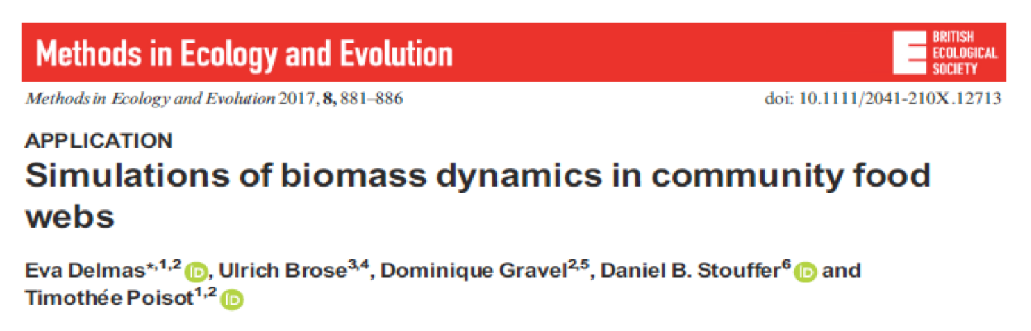
\includegraphics[height=1in]{intro_figs/Delmas2017.eps}

      \end{centering}

      \begin{itemize}
        \whitem {\color{white}Niche model webs}
        \whitem {\color{white}Links assigned based on biomasses}
        \whitem {\color{white}Link strengths = 1/number of prey}
      \end{itemize}

      \begin{itemize}
        \whitem {\color{white}Calculated species' roles}
      \end{itemize}

    \end{frame}

  \begin{frame}{Relating species roles to extinction risk}
      \begin{itemize}
        \item Simulated networks stable at equilibrium
        \item Webs with 50-100 species, connectance 0.02-0.2
        \item 100 simulated ATN networks for each combination
      \end{itemize}

      \begin{centering}

      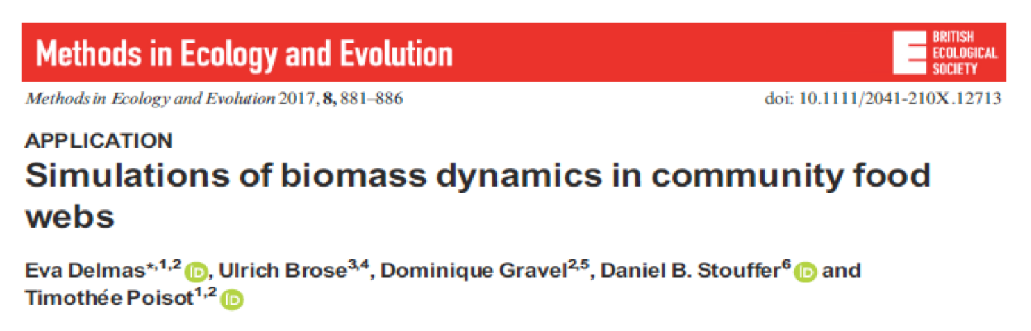
\includegraphics[height=1in]{intro_figs/Delmas2017.eps}

      \end{centering}

      \begin{itemize}
        \item Niche model webs
        \item Links assigned based on biomasses
        \item Link strengths = 1/number of prey
      \end{itemize}

      \begin{itemize}
        \whitem {\color{white}Calculated species' roles}
      \end{itemize}

    \end{frame}

  \begin{frame}{Relating species roles to extinction risk}
      \begin{itemize}
        \item Simulated networks stable at equilibrium
        \item Webs with 50-100 species, connectance 0.02-0.2
        \item 100 simulated ATN networks for each combination
      \end{itemize}

      \begin{centering}

      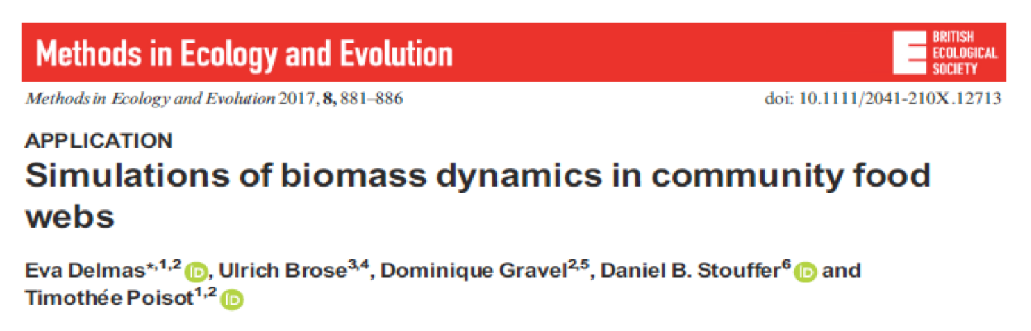
\includegraphics[height=1in]{intro_figs/Delmas2017.eps}

      \end{centering}

      \begin{itemize}
        \item Niche model webs
        \item Links assigned based on biomasses
        \item Link strengths = 1/number of prey
      \end{itemize}

      \begin{itemize}
        \item Calculated each species' role in each network
      \end{itemize}

    \end{frame}

\section*{Background - PCA of positions}

  \begin{frame}{Which positions are most important in species roles?}
    \begin{centering}
      \includegraphics[width=\textwidth]{../manuscript/figures/roles/roleplot_talk_axis.eps}
    \end{centering}
    
    {\color{DarkBlue}Motif roles for each species in each web, pre-disturbance}\\{\color{white}pppyyy}
    \end{frame}

  % \begin{frame}{Which positions are most important in species roles?}
  %   \begin{centering}
  %     \includegraphics[width=\textwidth]{../manuscript/figures/roles/roleplot_talk_Ax1.eps}
  %   \end{centering}

  %   {\color{DarkBlue}Axis 1: positions in apparent competition motif\\}
  %   {\color{white}Positions in one-way motifs strongly associated with PCA axes.}

  %   \end{frame}

  % \begin{frame}{Which positions are most important in species roles?}
  %   \begin{centering}
  %     \includegraphics[width=\textwidth]{../manuscript/figures/roles/roleplot_talk_Ax2.eps}
  %   \end{centering}

  %   {\color{DarkBlue}Axis 2: apparent competition prey vs. food chain predator\\}
  %   {\color{white}Positions in one-way motifs strongly associated with PCA axes.}

  %   \end{frame}

  % \begin{frame}{Which positions are most important in species roles?}
  %   \begin{centering}
  %     \includegraphics[width=\textwidth]{../manuscript/figures/roles/roleplot_talk_Ax3.eps}
  %   \end{centering}

  %   {\color{DarkBlue}Axis 3: apparent competition vs. other motifs\\}
  %   {\color{white}Positions in one-way motifs strongly associated with PCA axes.}

  %   \end{frame}

  \begin{frame}{Which positions are most important in species roles?}
    \begin{centering}
      \includegraphics[width=\textwidth]{../manuscript/figures/roles/roleplot_talk_allred.eps}
    \end{centering}

    Positions in one-way motifs strongly associated with PCA axes.\\
    {\color{white} One-way motifs associated with stability (Borrelli, Stouffer)}
    \end{frame}

  \begin{frame}{Positions in stable motifs define species roles}

    \begin{block}{Key motifs in six empirical marine webs:}

    \begin{centering}
      % \includegraphics[width=0.8\textwidth]{../manuscript/figures/roles/roleplot_talk_points.eps}

      \includegraphics[width=\textwidth]{Eklof_figs/PCA_positions.eps}

    \end{centering}

    \begin{itemize}
      \item Apparent competition
      \item Direct competition
      \item Three-species chains
    \end{itemize}
    \end{block}
    \vspace{-0.5cm}
    {\tiny Cirtwill \& Ekl\"{o}f, 2019, Ecology Letters}

    {\color{white}Stable motifs define roles (empirical and simulated webs)}\\
    {\color{white}But do stable motifs relate to vulnerability to extinction?}

    \end{frame}

  \begin{frame}{Positions in stable motifs define species roles}

    \begin{block}{Key motifs in six empirical marine webs:}

    \begin{centering}
      % \includegraphics[width=0.8\textwidth]{../manuscript/figures/roles/roleplot_talk_points.eps}

      \includegraphics[width=\textwidth]{Eklof_figs/PCA_positions.eps}

    \end{centering}

    \begin{itemize}
      \item Apparent competition
      \item Direct competition
      \item Three-species chains
    \end{itemize}
    \end{block}
    \vspace{-0.5cm}
    {\tiny Cirtwill \& Ekl\"{o}f, 2019, Ecology Letters}

    {\color{DarkBlue}Stable motifs define roles (empirical and simulated webs)}\\
    {\color{white}But do stable motifs relate to vulnerability to extinction?}

    \end{frame}

  \begin{frame}{Positions in stable motifs define species roles}

    \begin{block}{Key motifs in six empirical marine webs:}

    \begin{centering}
      % \includegraphics[width=0.8\textwidth]{../manuscript/figures/roles/roleplot_talk_points.eps}

      \includegraphics[width=\textwidth]{Eklof_figs/PCA_positions.eps}

    \end{centering}

    \begin{itemize}
      \item Apparent competition
      \item Direct competition
      \item Three-species chains
    \end{itemize}
    \end{block}
    \vspace{-0.5cm}
    {\tiny Cirtwill \& Ekl\"{o}f, 2019, Ecology Letters}

    {\color{DarkBlue}Stable motifs define roles (empirical and simulated webs)}\\
    {\color{DarkBlue}But do stable motifs relate to vulnerability to extinction?}

    \end{frame}


\section*{Methods - Measuring time to extinction}

  \begin{frame}{Determining vulnerability to extinction}

    \begin{textblock*}{7cm}(1cm,1.5cm)

      {\color{DarkBlue}Perturbation: species removal}

    \end{textblock*}

    \begin{textblock*}{5cm}(1cm,2.25cm)

      {\color{white}In each simulated network:}

      \begin{itemize}
        \whitem {\color{white}Remove a species}
        \whitem {\color{white}Simulate dynamics for 500 time steps}
        \whitem {\color{white}Record time step in which each species goes extinct}
        \whitem {\color{white}Reset to initial network}
        \whitem {\color{white}Repeat removing each species in turn}

      \end{itemize}

      \end{textblock*}

    \begin{textblock*}{5cm}(7cm,2cm)

      \includegraphics[width=5cm]{intro_figs/Otagoweb_remove3.eps}

      \end{textblock*}

    {\color{white} Response: each species' mean time to extinction\\
    But! potential variation between removals...}

    \end{frame}

  \begin{frame}{Determining vulnerability to extinction}

    \begin{textblock*}{7cm}(1cm,1.5cm)

      {\color{DarkBlue}Perturbation: species removal}

    \end{textblock*}

    \begin{textblock*}{5cm}(1cm,2.25cm)

      {\color{DarkBlue}In each simulated network:}

      \begin{itemize}
        \item Remove a species
        \whitem {\color{white}Simulate dynamics for 500 time steps}
        \whitem {\color{white}Record time step in which each species goes extinct}
        \whitem {\color{white}Reset to initial network}
        \whitem {\color{white}Repeat removing each species in turn}

      \end{itemize}

      \end{textblock*}

    \begin{textblock*}{5cm}(7cm,2cm)

      \includegraphics[width=5cm]{intro_figs/Otagoweb_remove3.eps}

      \end{textblock*}

    {\color{white} Response: each species' mean time to extinction\\
    But! potential variation between removals...}

    \end{frame}

  \begin{frame}{Determining vulnerability to extinction}
    \begin{textblock*}{7cm}(1cm,1.5cm)

      {\color{DarkBlue}Perturbation: species removal}

    \end{textblock*}

    \begin{textblock*}{5cm}(1cm,2.25cm) 

      {\color{DarkBlue}In each simulated network:}

      \begin{itemize}
        \item Remove a species
        \item Simulate dynamics for 500 time steps
        \item Record time step in which each species goes extinct
        \whitem {\color{white}Reset to initial network}
        \whitem {\color{white}Repeat removing each species in turn}

      \end{itemize}

      \end{textblock*}

    \begin{textblock*}{5cm}(7cm,2cm)

      \includegraphics[width=5cm]{intro_figs/Otagoweb_remove3.eps}

      \end{textblock*}

    \begin{textblock*}{1cm}(6.5cm,1,5cm)

      \includegraphics[width=1cm]{intro_figs/clock.eps}

      \end{textblock*}

    {\color{white} Response: each species' mean time to extinction\\
    But! potential variation between removals...}

    \end{frame}

  \begin{frame}{Determining vulnerability to extinction}
    \begin{textblock*}{7cm}(1cm,1.5cm)

      {\color{DarkBlue}Perturbation: species removal}

    \end{textblock*}

    \begin{textblock*}{5cm}(1cm,2.25cm)

      {\color{DarkBlue}In each simulated network:}

      \begin{itemize}
        \item Remove a species
        \item Simulate dynamics for 500 time steps
        \item Record time step in which each species goes extinct
        \item Reset to initial network
        \whitem {\color{white}Repeat removing each species in turn}

      \end{itemize}

      \end{textblock*}

    \begin{textblock*}{5cm}(7cm,2cm)

      \includegraphics[width=5cm]{intro_figs/Otagoweb_minimal.eps}

      \end{textblock*}

    % \begin{textblock*}{1cm}(6.5cm,1,5cm)

    %   \includegraphics[width=1cm]{intro_figs/clock.eps}

    %   \end{textblock*}

    {\color{white} Response: each species' mean time to extinction\\
    But! potential variation between removals...}

    \end{frame}

  \begin{frame}{Determining vulnerability to extinction}

    \begin{textblock*}{7cm}(1cm,1.5cm)

      {\color{DarkBlue}Perturbation: species removal}

    \end{textblock*}

    \begin{textblock*}{5cm}(1cm,2.25cm)

      {\color{DarkBlue}In each simulated network:}

      \begin{itemize}
        \item Remove a species
        \item Simulate dynamics for 500 time steps
        \item Record time step in which each species goes extinct
        \item Reset to initial network
        \item Repeat removing each species in turn

      \end{itemize}

      \end{textblock*}

    \begin{textblock*}{5cm}(7cm,2cm)

      \includegraphics[width=5cm]{intro_figs/Otagoweb_remove2.eps}

      \end{textblock*}

    \begin{textblock*}{1cm}(6.5cm,1,5cm)

      \includegraphics[width=1cm]{intro_figs/clock.eps}

      \end{textblock*}

    {\color{white} Response: each species' mean time to extinction\\
    But! potential variation between removals...}

    \end{frame}

  \begin{frame}{Determining vulnerability to extinction}

    \begin{textblock*}{7cm}(1cm,1.5cm)

      {\color{DarkBlue}Perturbation: species removal}

    \end{textblock*}

    \begin{textblock*}{5cm}(1cm,2.25cm)

      {\color{DarkBlue}In each simulated network:}

      \begin{itemize}
        \item Remove a species
        \item Simulate dynamics for 500 time steps
        \item Record time step in which each species goes extinct
        \item Reset to initial network
        \item Repeat removing each species in turn

      \end{itemize}

      \end{textblock*}

    \begin{textblock*}{5cm}(7cm,2cm)

      \includegraphics[width=5cm]{intro_figs/Otagoweb_remove2.eps}

      \end{textblock*}

    \begin{textblock*}{10cm}(1cm,8cm)
      {\color{DarkBlue} Response: each species' mean time to extinction}\\
      {\color{white}But! potential variation between removals...}
      \end{textblock*}

    \end{frame}

  \begin{frame}{Determining vulnerability to extinction}

    \begin{textblock*}{7cm}(1cm,1.5cm)

      {\color{DarkBlue}Perturbation: species removal}

    \end{textblock*}

    \begin{textblock*}{5cm}(1cm,2.25cm)

      {\color{DarkBlue}In each simulated network:}

      \begin{itemize}
        \item Remove a species
        \item Simulate dynamics for 500 time steps
        \item Record time step in which each species goes extinct
        \item Reset to initial network
        \item Repeat removing each species in turn

      \end{itemize}

      \end{textblock*}

    \begin{textblock*}{5cm}(7cm,2cm)

      \includegraphics[width=5cm]{intro_figs/Otagoweb_remove2.eps}

      \end{textblock*}

    \begin{textblock*}{10cm}(1cm,8cm)
      {\color{DarkBlue} Response: each species' mean time to extinction.\\
      But! potential variation between removals...}
      \end{textblock*}

    \end{frame}

  \begin{frame}{Determining vulnerability to extinction}

    \begin{block}{Is time to extinction correlated across removals?}

    \vspace{0.2cm}

    \begin{centering}

      \includegraphics[width=0.9\textwidth]{../manuscript/figures/extinction_order/extorder_correlations_talk_axis.eps}
    
      \end{centering}

    \end{block}

    \begin{itemize}
      \item $R^2 \approx$ species, connectance, network
      \whitem {\color{white}Correlation stronger in larger, more-connected webs}
      \whitem {\color{white}$p$\textless0.001}
    \end{itemize}

    \end{frame}

  % \begin{frame}{Determining vulnerability to extinction}

  %   \begin{block}{Is time to extinction correlated across removals?}

  %   \vspace{0.2cm}

  %   \begin{centering}
    
  %     \includegraphics[width=0.9\textwidth]{../manuscript/figures/extinction_order/extorder_correlations_talk_point.eps}
    
  %     \end{centering}

  %   \end{block}

  %   \begin{itemize}
  %     \whitem {\color{white}Times to extinction highly correlated}
  %     \whitem {\color{white}Correlation stronger in larger, more-connected webs}
  %     \whitem {\color{white}$p$\textless0.001}
  %   \end{itemize}

  %   \end{frame}

  \begin{frame}{Determining vulnerability to extinction}

    \begin{block}{Is time to extinction correlated across removals?}

    \vspace{0.2cm}

    \begin{centering}
    
      \includegraphics[width=0.9\textwidth]{../manuscript/figures/extinction_order/extorder_correlations_talk_full.eps}
    
      \end{centering}

    \end{block}

    \begin{itemize}
      \item Times to extinction highly correlated
      \whitem {\color{white}Correlation stronger in larger, more-connected webs}
      \whitem {\color{white}$p$\textless0.001}
    \end{itemize}

    \end{frame}

  \begin{frame}{Determining vulnerability to extinction}

    \begin{block}{Is time to extinction correlated across removals?}

    \vspace{0.2cm}

    \begin{centering}
    
      \includegraphics[width=0.9\textwidth]{../manuscript/figures/extinction_order/extorder_correlations_talk_full.eps}
    
      \end{centering}

    \end{block}

    \begin{itemize}
      \item Times to extinction highly correlated
      \item Correlation stronger in larger, more-connected webs
      \item $p$\textless0.001
    \end{itemize}

    \end{frame}

\section*{Results - Permanova} % Will need to figure out the methods stuff later, eh?

  \begin{frame}{Is time to extinction related to species roles?}
    \begin{itemize}
      \item PERMANOVA of mean time to extinction vs. initial role
      \item One PERMANOVA per combination of S,C
    \end{itemize}

    \begin{centering}
      \includegraphics[width=\textwidth]{../manuscript/figures/extinction_order/permanova_summary_talk_axis.eps}
    \end{centering}

    \begin{itemize}
      \whitem {\color{white}Individually, each PERMANOVA significant}
      \whitem {\color{white}After Bonferroni correction, none significant}
      \whitem {\color{white}Results indicative, but need backup}
    \end{itemize}
    
    \end{frame}

  \begin{frame}{Is time to extinction related to species roles?}
    \begin{itemize}
      \item PERMANOVA of mean time to extinction vs. initial role
      \item One PERMANOVA per combination of S,C
    \end{itemize}
    
    \begin{centering}
      \includegraphics[width=\textwidth]{../manuscript/figures/extinction_order/permanova_summary_talk_full.eps}
    \end{centering}
    
    \begin{itemize}
      \whitem {\color{white}Individually, each PERMANOVA significant}
      \whitem {\color{white}After Bonferroni correction, none significant}
      \whitem {\color{white}Results indicative, but need backup}
    \end{itemize}
    
    \end{frame}

  \begin{frame}{Is time to extinction related to species roles?}
    \begin{itemize}
      \item PERMANOVA of mean time to extinction vs. initial role
      \item One PERMANOVA per combination of S,C
    \end{itemize}
    
    \begin{centering}
      \includegraphics[width=\textwidth]{../manuscript/figures/extinction_order/permanova_summary_talk_full.eps}
    \end{centering}
    
    \begin{itemize}
      \item Individually, each PERMANOVA significant
      \whitem {\color{white}After Bonferroni correction, none significant}
      \whitem {\color{white}Results indicative, but need backup}
    \end{itemize}

    \end{frame}

  \begin{frame}{Is time to extinction related to species roles?}
    \begin{itemize}
      \item PERMANOVA of mean time to extinction vs. initial role
      \item One PERMANOVA per combination of S,C
    \end{itemize}
    
    \begin{centering}
      \includegraphics[width=\textwidth]{../manuscript/figures/extinction_order/permanova_summary_talk_full.eps}
    \end{centering}
    
    {\color{white}
    \begin{itemize}
      \item Individually, each PERMANOVA significant
      \item After Bonferroni correction, none significant
      \whitem {\color{white}Results indicative, but need backup}
    \end{itemize}
    }

    \end{frame}

  \begin{frame}{Is time to extinction related to species roles?}
    \begin{itemize}
      \item PERMANOVA of mean time to extinction vs. initial role
      \item One PERMANOVA per combination of S,C
    \end{itemize}
    
    \begin{centering}
      \includegraphics[width=\textwidth]{../manuscript/figures/extinction_order/permanova_summary_talk_full.eps}
    \end{centering}
    
    \begin{itemize}
      \item Individually, each PERMANOVA significant
      \item After Bonferroni correction, none significant
      \item Results indicative, but need backup
    \end{itemize}

    \end{frame}

% \section*{Methods: lmers - PCA}

%   \begin{frame}{Linking time to extinction and roles: PCA axes}

%     {\color{DarkBlue}
%     \begin{equation*}
%     \tau_{in} \approx \rho_i + \sigma_n + \chi_n + \rho_{i}\sigma_{n} + \rho_{i}\chi_{n} + \sigma_{n}\chi_{n} + \rho_{i}\sigma_{n}\chi_{n}
%     \end{equation*}
%     }

%     \begin{itemize}
%       \item $\tau$: mean time to extinction
%       \item $\rho$: loading on PCA axis (scaled)
%       \item $\sigma$: species richness (scaled)
%       \item $\chi$: connectance (scaled)
%     \end{itemize}

%     \end{frame}

% \section*{Results: PCA lmers}

%   \begin{frame}{Is mean time to extinction related to major role axes?}
%     \begin{centering}
%       \includegraphics[width=\textwidth]{../manuscript/figures/extinction_order/PCA_position_lmer_summary_talk_axis.eps}
%     \end{centering}

%     {\color{white}Higher values on Axis 1 -> longer times to extinction, 
%     \\especially in smaller webs}

%     \end{frame}

%   \begin{frame}{Is mean time to extinction related to major role axes?}
%     \begin{centering}
%       \includegraphics[width=\textwidth]{../manuscript/figures/extinction_order/PCA_position_lmer_summary_talk_single.eps}
%     \end{centering}

%     Higher values on Axis 1 -> longer times to extinction, 
%     \\especially in smaller and lower-connectance webs

%     \end{frame}

%   \begin{frame}{Is mean time to extinction related to major role axes?}
%     \begin{centering}
%       \includegraphics[width=\textwidth]{../manuscript/figures/extinction_order/PCA_position_lmer_summary_talk_two.eps}
%     \end{centering}

%     Higher values on Axis 2 -> slightly lower times to extinction,
%     \\except in large, low-connectance webs

%     \end{frame}

%   \begin{frame}{Is mean time to extinction related to major role axes?}
%     \begin{centering}
%       \includegraphics[width=\textwidth]{../manuscript/figures/extinction_order/PCA_position_lmer_summary_talk_full.eps}
%     \end{centering}

%     Higher values on Axis 3 -> longer times to extinction,
%     \\except in large, low-connectance webs

%     \end{frame}


%   \begin{frame}{Mean time to extinction IS related to major role axes}
%     \begin{centering}
%       \includegraphics[width=\textwidth]{../manuscript/figures/extinction_order/PCA_position_lmer_summary_talk_full.eps}
%     \end{centering}

%     Relationship dependent on size, connectance on web.
%     \\Association with multiple motifs -> difficult to interpret

%     \end{frame}

\section*{Motif participation LMERs}

  \begin{frame}{Linking time to extinction and roles: motifs}

    % \vspace{-0.25cm}
    A more specific measure: motif participation

    \vspace{-0.4cm}
    {\color{DarkBlue}
    \begin{equation*}
    \tau_{in} \approx \mu_i + \sigma_n + \chi_n + \mu_{i}\sigma_{n} + \mu_{i}\chi_{n} + \sigma_{n}\chi_{n} + \mu_{i}\sigma_{n}\chi_{n} + Network
    \end{equation*}
    }
    \vspace{-0.4cm}
    \begin{itemize}
      \item $\tau$: mean time to extinction
      \item $\mu$: times participating in motif (scaled)
      \item $\sigma$: species richness (scaled)
      \item $\chi$: connectance (scaled)
    \end{itemize}

    \begin{centering}

      \includegraphics[height=2.5cm]{intro_figs/stable_motifs_and_positions.eps}

    \end{centering}

    {\color{white}Focusing on: chain, apparent \& direct competition, omnivory}


    \end{frame}

  \begin{frame}{Linking time to extinction and roles: motifs}

    A more specific measure: motif participation

    \vspace{-0.4cm}
    {\color{DarkBlue}
    \begin{equation*}
    \tau_{in} \approx \mu_i + \sigma_n + \chi_n + \mu_{i}\sigma_{n} + \mu_{i}\chi_{n} + \sigma_{n}\chi_{n} + \mu_{i}\sigma_{n}\chi_{n} + Network
    \end{equation*}
    }
    \vspace{-0.4cm}
    \begin{itemize}
      \item $\tau$: mean time to extinction
      \item $\mu$: times participating in motif (scaled)
      \item $\sigma$: species richness (scaled)
      \item $\chi$: connectance (scaled)
    \end{itemize}

    \begin{centering}

      \includegraphics[height=2.5cm]{intro_figs/stable_motifs_and_positions.eps}

    \end{centering}

    {\color{DarkBlue}Focusing on: chain, apparent \& direct competition, omnivory}

    \end{frame}

  \begin{frame}{Is time to extinction related to motif participation?}

    \begin{centering}

      \includegraphics[height=.65\textheight]{../manuscript/figures/extinction_order/motif_lmer_summary_talk_axis.eps}
    
    \end{centering}

    {\color{white}Participating in food chains -> slower time to extinction\\
    especially in smaller, less connected webs}

    \end{frame}

  \begin{frame}{Is time to extinction related to motif participation?}

    \begin{centering}

      \includegraphics[height=.65\textheight]{../manuscript/figures/extinction_order/motif_lmer_summary_talk_point.eps}

    \end{centering}

    Participating in food chains -> slower time to extinction\\
    {\color{white}especially in smaller, less connected webs}

    \end{frame}

  \begin{frame}{Is time to extinction related to motif participation?}

    \begin{centering}

      \includegraphics[height=.65\textheight]{../manuscript/figures/extinction_order/motif_lmer_summary_talk_single.eps}

    \end{centering}

    Participating in food chains -> slower time to extinction,\\
    especially in smaller, less connected webs

    \end{frame}

  \begin{frame}{Is time to extinction related to motif participation?}

    \begin{centering}

      \includegraphics[height=.65\textheight]{../manuscript/figures/extinction_order/motif_lmer_summary_talk_full.eps}

    \end{centering}

    Participating in stable motifs -> slower time to extinction,\\
    especially in smaller, less connected webs

    \end{frame}

  \begin{frame}{Time to extinction IS related to motif participation}

    \begin{centering}

      \includegraphics[height=.65\textheight]{../manuscript/figures/extinction_order/motif_lmer_summary_talk_full.eps}


    {\color{DarkBlue}Easier to identify links than dynamics, faster diagnosis\\}
    {\color{white}Motif roles/participation allow rapid triage}
    \end{centering}

    \end{frame}


\section*{Summary}

  % \begin{frame}{Recap: one-way motifs define roles}

  %   \begin{centering}
  %     \includegraphics[width=\textwidth]{../manuscript/figures/roles/roleplot_talk_allred.eps}
  %   \end{centering}

  %   \begin{itemize}
  %     \item Stable motifs are associated with major role axes
  %     \item In simulated and empirical webs!
  %   \end{itemize}

  %   \end{frame}

  % \begin{frame}{Recap: vulnerability is consistent over removals}

  %   \begin{centering}
  %     \includegraphics[width=\textwidth]{../manuscript/figures/extinction_order/extorder_correlations_talk_full.eps}
  %   \end{centering}

  %   \begin{itemize}
  %     \item Stable motifs are associated with major role axes
  %     \item In simulated and empirical webs!
  %     \item Time to extinction is consistent over removals
  %   \end{itemize}

  %   \end{frame}

  % \begin{frame}{Recap: species roles do predict extinction risk}

  %   \begin{center}
  %     \includegraphics[height=.65\textheight]{../manuscript/figures/extinction_order/motif_lmer_summary_talk_full.eps}
  %   \end{center}

  %   \vspace{-0.5cm}
  %   \begin{itemize}
  %     \item Time to extinction is related to species roles
  %     \item Participating in stable motifs slows time to extinction
  %   \end{itemize}

  %   \end{frame}

  \begin{frame}{Next steps:}

    \begin{textblock*}{.5\textwidth}(6cm,1.5cm)
    \begin{center}
      \includegraphics[width=\textwidth]{../manuscript/figures/extinction_order/motif_lmer_summary_talk_full.eps}
    \end{center}
    \end{textblock*}

    \begin{textblock*}{.5\textwidth}(0.5cm,2cm)
      \begin{itemize}
        \item Smaller perturbations (biomass reduction)
        \item Perturbation of groups of species
        \item Relationships between focal and removed species?
        \whitem {\color{white}Suggestions?}
      \end{itemize}
    \end{textblock*}

    \end{frame}

  \begin{frame}{Next steps:}

    \begin{textblock*}{.5\textwidth}(6cm,1.5cm)
    \begin{center}
      \includegraphics[width=\textwidth]{../manuscript/figures/extinction_order/motif_lmer_summary_talk_full.eps}
    \end{center}
    \end{textblock*}

    \begin{textblock*}{.5\textwidth}(0.5cm,2cm)
      \begin{itemize}
        \item Smaller perturbations (biomass reduction)
        \item Perturbation of groups of species
        \item Relationships between focal and removed species?
        \item Suggestions?
      \end{itemize}
    \end{textblock*}

    \end{frame}

  \begin{frame}{Thanks to:}
      \begin{textblock*}{3cm}(1cm,1.5cm)
          \includegraphics[width=3cm]{intro_figs/SU_logo.eps} \\
          \vspace{0.2cm}
          \includegraphics[width=3cm]{intro_figs/SLU_logo.eps} 
        \end{textblock*} 

      \begin{textblock*}{4cm}(4.5cm,2.5cm)
          \includegraphics[height=4cm]{intro_figs/happyKate.eps} 
        \end{textblock*} 

      \begin{textblock*}{3cm}(8cm,1.5cm)
          \includegraphics[width=3cm]{intro_figs/Poisotlab.eps} \\
          \vspace{0.2cm}
          \includegraphics[width=3cm]{intro_figs/DBS.eps} 
        \end{textblock*} 


      \begin{textblock*}{10cm}(1cm,7.5cm)
        \includegraphics[width=10cm]{intro_figs/package.eps}
        \end{textblock*} 
    \end{frame}

  \begin{frame}{Species roles do predict extinction risk}

    \begin{textblock*}{5cm}(1cm,1.5cm)
      \begin{center}
      \vspace{-0.5cm}
      \includegraphics[width=.9\textwidth]{../manuscript/figures/extinction_order/extorder_correlations_talk_full.eps}

      \end{center}
    \end{textblock*}

    \begin{textblock*}{5cm}(1cm,4cm)
      \includegraphics[width=\textwidth]{../manuscript/figures/extinction_order/permanova_summary_talk_full.eps}
    \end{textblock*}

    \begin{textblock*}{5cm}(7cm,1.5cm)
      \includegraphics[width=\textwidth]{../manuscript/figures/extinction_order/motif_lmer_summary_talk_full.eps}
    \end{textblock*}

    \begin{textblock*}{10cm}(1cm,6cm)

    \begin{itemize}
      \item Stable motifs are associated with major role axes
      \item In simulated and empirical webs!
      \item Time to extinction is consistent over removals
      \item Time to extinction is related to species roles
      \item Participating in stable motifs slows time to extinction
    \end{itemize}
    \end{textblock*}

    \end{frame}

\end{document}

